% define the type of document I want to make (article), set 12pt font and letter-sized paper
\documentclass[12pt, letterpaper]{article}

% the natbib package lets me use extra citation commands, authoryear sorts bibliography by author last name, then year of publication
\usepackage[authoryear]{natbib}
% the hyperref package lets me insert a hyperlink, and makes table of contents and references clickable
\usepackage{hyperref}
% wasysym lets me insert a smiley/frowny face
\usepackage{wasysym}
% graphicx allows....graphics
\usepackage{graphicx}
% tikz-feynman lets you easily draw Feynman diagrams. Explained in the section "Something New and Exciting"
\usepackage[compat=1.1.0]{tikz-feynman}



% enter the document environment to begin!
\begin{document}

% set the title
\title{Homework 1 - PHYS 5391}
% set author
\author{Elizabeth Vandegriff}
% set date as current date
\date{\today}

% make the above title/author/date visible
\maketitle
% leave the rest of the title page blank
\newpage
% create a table of contents based on the sections I define throughout the doc
\tableofcontents
% start sections on new page after table of contents
\newpage

% first section!
\section{Programming Experience}

% A section dedicated to your current programming experience. Discuss what languages you have used in the past, what types of tasks you are comfortable performing, and what languages and tasks you would like to learn. If there are any texts that you found particularly helpful and would strongly recommend, be sure to cite them in your bibliography.

My first ever ``programming'' experience was in high school, where I  used a program called \href{https://www.alice.org/}{Alice} to make a figure skater complete a very complex and mind-bending skating routine. I did this completely on my own, by trial and error, and had a blast.

In undergrad, I started using Mathematica, then took my first ever programming class, where I learned basic Python. I don't remember if we did much object oriented work at all, so clearly if we did, it didn't stick. In 2016 I did some development of the spacepy pycdf capabilities at the University of New Hampshire (UNH) in preparation for the Parker Solar Probe mission. In 2017 I participated in a theoretical neuclear astronomy research group where I taught myself basic C for the purpose of visualizing simulations of neutron star crusts. I took a C++ class later on, but I have not used C or C++ since then, so it would take me a little while to get back up to speed. In addition, I used MatLab in multiple math classes, as well as a computer imaging class. Throughout undergrad I used \LaTeX to write lab reports, class project reports, and my senior project.

In 2018/2019 I used Python to analyze LANL GEO data, and starting in Fall of 2019, I have been using Python to analyze Space Weather Modeling Framework (SWMF) runs.

I am comfortable with writing (sloppy) Python, and I am pretty good at learning new languages, so I am excited to learn Fortran. I want to get better at structuring and documenting my code, as well as learning more about object oriented programming in Python and what situations it is best suited for.

The tools I used to learn were either the Internet, lectures, trial and error, or a combination of all these, so I haven't used any specific texts that I could recommend.

% enter a new section
\section{Programming Environment}

% Describe your programming environment in terms of operating system, text/code editor, and access to a command line terminal. I want to know how you'll be doing work for this class. Are you using a personal Windows laptop? Will you be relying on CAEN computers? Do you have access to the appropriate tools?

I am working in a Macintosh operating system, specifically Mac OS Mojave (version 10.14.6) on the laptop loaned to me for research at UTA. I am using XQuartz as my command line terminal, and a combination of Emacs and Spyder for text/code editing. Other relevant environment considerations: I do not have a printer, and I miss my office-mate Christian \frownie{}.

% yet another section
\section{Favorite Equation}

% A section where you select your favorite physical law/equation, list it explicitly, and describe in words what it means. Describe each term in detail. Include a table that lists each variable and its meaning. Ensure that your equation has a number and that you reference it properly, e.g. \Equation 1 shows that...". Use the nref syntax such that if I add an equation randomly in your document, it will not ruin your referencing.

My favorite equation at this moment in time is the magnetohydrodynamics (MHD) momentum equation, given by Equation \ref{eq:1}

% enter environment for a referencable math equation
\begin{equation}
  % provide label so it can be referenced
  \label{eq:1}
  % components of the actual equation
  \rho \frac{d \vec{u}}{dt} = - \nabla P + \vec{J} \times \vec{B}
% leave the equation environment
\end{equation}

This equation is basically the $\vec{F}=m\vec{a}$ of the MHD world, and shows that the sum of the negative pressure force and the Lorentz force is equal to the mass density times the acceleration of the plasma. This equation holds for isotropic pressure cases.

Let's break this equation down into components in Table \ref{tab:1}:

% enter table environment
% ht! sets the table location directly where I make it in the document
\begin{table}[ht!]
  % puts table in center of the page
  \centering
  % enter tabular environment, left aligned left col, centered right col
  % | characters indicate which cols to place vertical lines between
  \begin{tabular}{|l|c|}
    % add a horizontal line
    \hline
    % define the two columns
    Variable & Meaning\\
    % another horizontal line
    \hline
    % put each variable in table using inline math notation
    $\rho$ & Plasma mass density\\ 
    $\frac{d \vec{u}}{dt}$ & Time derivative of the plasma flow speed\\
    $\nabla P$ & Plasma pressure gradient\\
    $\vec{J}$ & Current density\\
    $\vec{B}$ & Magnetic field\\
    % another horizontal line
    \hline
  % leave tabular environment
  \end{tabular}
  % table caption
  \caption{Description of variables in MHD momentum equation.}
  % label so I can reference table
  \label{tab:1}
% exit out of table environment
\end{table}

% another section
\section{Thoughts on Example Doc}

% A section where you comment on the example document you studied for Questions 2 and 3. Was it clear? Was it accurate? Was it complete? Your input will be used to refine it.

I liked the example document, and I definitely used it as a reference for things I did not know (or forgot) how to do. Honestly, I can't think of anything I would change, I think it's a great guide that doesn't have too many details but goes over all the most common/essential items.

% another section
\section{Article Summaries}

% A section where you select three or more scholarly articles you have read and briefly summarize them (one or two sentences per article). Be sure to properly cite each article in your bibliography!

Each of the following subsections gives a short summary of one scholarly article that I have recently read. 


% begin a subsection
\subsection{On the regional variability of dB/dt and its significance to GIC}

% in-text citation
\citet[]{Dimmock2020} describes the differences in magnetometer readings over small scales (~500km), possible causes, and impacts on modeling. Scientists are interested in modeling and predicting these variations because they affect ground conducting systems such as power lines.


% begin a subsection
\subsection{Supermagnetosonic subsolar magnetosheath jets and their effects: From the solar wind to the ionospheric convection}

\citet[]{Hietala2012} presents a study of spacecraft observations of high speed jets in the magnetosheath, as well as their size and effects in various regions of the magnetosheath, magnetosphere, and ionosphere for the March 17, 2007 event.


% begin a subsection
\subsection{Role of magnetosheath force balance in regulating the dayside reconnection potential}

Using both simulation and spacecraft data, \citet[]{Lopez2010} studies the ionospheric potentials that result from the full range of possibilities for solar wind conditions, including ionospheric potential saturation, and presents force balance in the magnetosheath as the main regulator of geoeffective length. 


% begin a subsection
\subsection{Defining Radiation Belt Enhancement Events Based on Probability Distributions}

\citet[]{Reeves2020} outlines a new method of defining space weather events by examining ion and electron flux data from the LANL geosynchronous satellites from 1989 through 2018. Examining frequency of events per solar cycle as a function of event flux threshold yields a determination of magnitude for moderate (100 occurrences per cycle), strong (10 occurrences per cycle), and intense (1 occurrence per cycle) events, which is then applied to data from the Van Allen Probes mission and can be applied to other datasets.

% another section
\section{Image and Explanation}

% A section where you select a random picture that you obtain from the Internet and include it in the document. Caption it, then include a paragraph that describes and references it properly (e.g., \Figure 1 illustrates how a dog would answer a phone...").

% enter the figure environment
\begin{figure}[!ht]
  %center the figure
  \centering
  % insert figure using the filename
  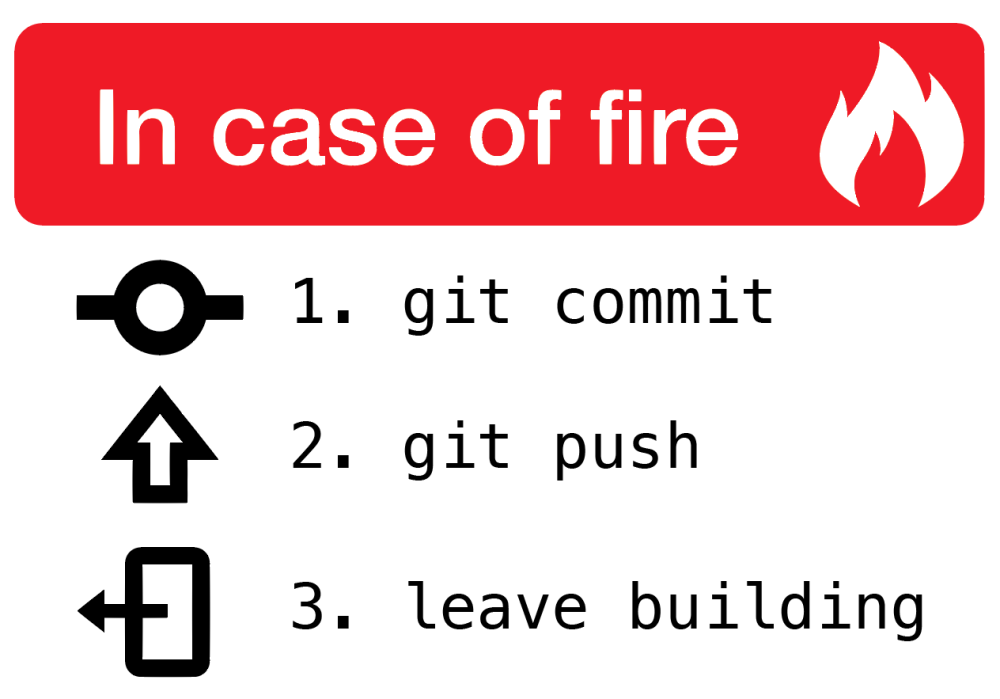
\includegraphics[width=8cm]{meme.png}
  % caption that will appear in the document
  \caption{In case of fire.}
  % label so figure can be referenced
  \label{fig:meme}
  %exit the figure environment
\end{figure}

Figure \ref{fig:meme} shows what to do in the case of a fire in the building while you are making changes to a repository. For legal reasons, this is a joke.


% another section
\section{Something New and Exciting}

% Perform some task not covered in the example document. For example, split your document into two columns, insert some colored text in the document, create clickable-hyperlinks, or customize the document's layout. You will need to research what to do and how to do it. Include a section that says specifically what task you performed and how you were able to achieve it. I want you to teach me how to do what you did.

Let's make our very own Feynman diagram right in the \LaTeX environment! Figure \ref{fig:feynman} shows the decay of the top quark, and this section outlines how to recreate it.

% enter figure environment, make figure appear RIGHT HERE
\begin{figure}[ht!]
  % center it, brah
  \centering
  % enter line-drawing environment
  \begin{tikzpicture}
    % enter feynman environment
    \begin{feynman}
      % define initial vertex of decay
      \vertex (a) {\(t\)};
      % define other vertices in relation to each other
      \vertex [right=of a] (b);
      \vertex [above right=of b] (f1) {\(b\)};
      \vertex [below right=of b] (c);
      \vertex [above right=of c] (f2) {\(\overline \ell\)};
      \vertex [below right=of c] (f3) {\(\nu_{\ell}\)}; 

      % enter diagram environment to specify particle types, edges, labels
      \diagram* {
        (a) -- [fermion] (b) -- [fermion] (f1),
        (b) -- [boson, edge label'=\(W^{+}\)] (c),
        (c) -- [anti fermion] (f2),
        (c) -- [fermion] (f3),
      };
    % exit feynman environment
    \end{feynman}
  % exit tikzpicture environment
  \end{tikzpicture}
  % cool caption
  \caption{Decay of the top quark, involving a virtual $W$ particle, a bottom quark, a lepton, and a neutrino.}
  % cool label
  \label{fig:feynman}
% exit figure environment
\end{figure}

There are several ways to make this figure, but the easiest is by using the Ti\textit{k}Z-Feynman package as follows:

% quote to show exact package import command
\begin{quote}
% make sure LaTeX doesn't try to re-import the package
\begin{verbatim}
\usepackage[compat=1.1.0]{tikz-feynman}
\end{verbatim}
% leave quote environment
\end{quote}

where {\tt [compat=1.1.0]} sets the version of the package to a constant so your drawing doesn't get ruined by a future update of the package. \href{https://www.overleaf.com/learn/latex/feynman\_diagrams}{This link} gives a good explanation of how to use the package, and is based off \citet[]{Ellis2016}

Because this decay is complicated I had to use manual placement of the vertices (outlined in \citet[Sec 2.4.3]{Ellis2016}) rather than the more simple diagram options available. Comments in my \texttt{.tex} file show how I constructed the Feynman diagram using the manual placement technique.
% adding a space to make the next paragraph stand out
\vspace{4mm}
% adding a non-indented note in italics with breaks for some typewriter text
\noindent \emph{\textbf{Note:} Compiling the TikZ-Feynman package with} \texttt{pdflatex} \emph{gives several warnings, but seems to work fine for my particular diagram. Compiling with} \texttt{lualatex} \emph{is recommended by the developer and works without issue.}



% puts bibliography on new page
\clearpage
% make sure bibliography ends up in the table of contents
\addcontentsline{toc}{section}{Bibliography}

% choosing the built-in bibliography style
\bibliographystyle{plainnat}
% choosing which .bib file to read bibliography from
\bibliography{hw1_5391_vandegriff}

% leave the document environment, because we're done!
\end{document}
